This taxonomy of dialogue acts is derived from DIT++\cite{bunt2009dit++}.

\subsection{Concept definitions}
\label{subsec:dialogue_acts}

\subsubsection{Dialogue acts}

\begin{figure}
	\caption{Meta-model}
	\centering
	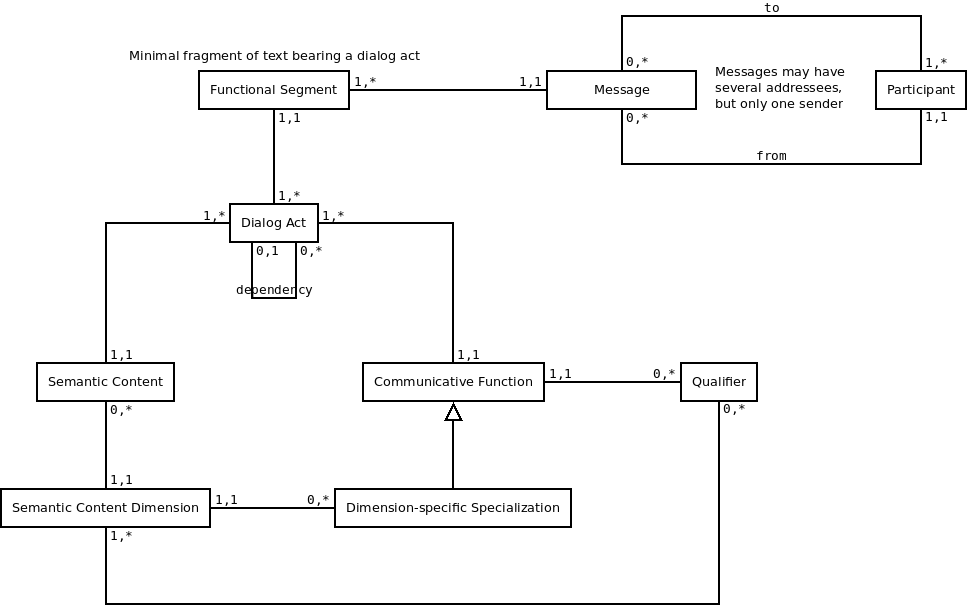
\includegraphics[keepaspectratio,width=0.6\paperwidth]{figures/objects.png}
	\label{fig:metaModel}
\end{figure}

In the "information-state update" (also know as "context-change") approach to dialogue analysis, dialogue acts are interpreted as update operations applied to the information states of the interacting participants \cite{traum2003information,bunt2011semantics}. In this perspective, they are defined here as the conjunction of two components: a \textit{semantic content} and a \textit{communicative function} (see figure \ref{fig:fundamentalTaxonomies}).

The former, the semantic content, specifies the objects, propositions, and all the things that the dialogue act is about, and therefore contains all the information used in the update operation. The latter, the communicative function, specifies the way the dialogue act is intended to impact the information state of the addressee. For example, the utterance "do you know what time it is?" is about the time that it is - that's its semantic content - but its communicative function could be either a genuine question (the speaker doesn't know the time but wants to find out) or a reproach (the speaker noticed the addressee is late and is upset about it).

A functional segment is defined as the minimal fragment of text bearing a dialogue act and is hereafter used interchangeably with the term "utterance".

\subsubsection{Dimensions in dialogue act annotation}

Human communication is a complex activity. In functional conversations, there is often a certain activity or task which the participants want to perform through the dialogue and as a result is the focus most interactions. In conversations bearing requests for assistance, this task is to solve problems. However, people do not communicate only to reach the formal objectives of the conversation, they also constantly monitor the communicative process, synchronize their mutual understanding through feedback utterances, respect social conventions such as greeting and thanking, etc. Often, utterances can be multifunctional and may serve several purposes related to several of these things. For example, in the following exchange:

\begin{enumerate}
	\item P1: Comment est ce que j'installe Dia ?
	\item P2: Tout simplement : apt-get install dia
	\item P1: Ça me dit permission non accordée je fais quoi ? 
	\item P3: Essaye avec sudo devant la commande
	\item P1: C'est bon merci !
\end{enumerate}

In the third utterance, participant 1 does two things: firstly, he informs his audience that he ran into an issue, and, secondly, he asks for further instructions. In the fifth utterance, he does two things again: he signifies that his problem is solved, and he also thanks the participants that helped him.

Such multi-functionality implies that accurate annotation of utterances with dialogue act information calls for the assignment of more than one tag to an utterance. This process is called "multi-label annotation". However in most multi-label schemes, only a small percentage of possible tag combinations are actually used, due to the fact that many tags are in fact mutually exclusive. This is an issue because it makes both human annotation and machine classification harder by unnecessarily increasing the task's complexity.

Here, like in DIT++, we guide annotators and classification algorithms in not considering impossible label combinations by the use of a multidimensional annotation scheme \cite{bunt2006dimensions}. The scheme allows each utterance to be annotated with one of 14 mutually exclusive tags per \textit{semantic dimension}. Semantic dimensions are defined as the different areas within which dialogue acts can be semantically categorized.

For example, if the communicative function of the fragment "C'est bon merci !" for a dimension called "social management" is "express gratitude", it cannot be any other in the same dimension, but it can be another in a different one, like "indicate problem solved" in the dimension "task management" for example.

\subsection{Taxonomy}

\subsubsection{Dimensions}

For this scheme, we define six semantic dimensions:

\begin{itemize}
	\item Communication: dialogue acts about the communication process (e.g. \textit{"J'ai fait une faute de frappe dans mon précédent mail c'est grep pas gret"})
	\item Discourse: dialogue acts affect both the discourse's structure and the topics discussed (e.g. \textit{"Avant de vous expliquer mon problème, j'ai un coup de gueule à faire passer"})
	\item Social Obligations: dialogue acts that take care of social conventions such as thanks, greetings, apologies etc. (e.g. \textit{"Merci beaucoup !!!!"})
	\item Auto Feedback: dialogue acts related to the speaker's own processing of an utterance (e.g. \textit{"Perso j'ai rien compris"})
	\item Allo Feedback: dialogue acts related to the addressee(s)'(s) processing of an utterance (e.g. \textit{"Je sais pas si je suis très clair...?"})
	\item Task: dialogue acts that bring information about the task's objects, i.e. problems, solutions, goals, user profiles, contexts, etc. (e.g. \textit{"Mon problème c'est que j'ai même pas l'icône dans le systray"})
\end{itemize}

\subsubsection{Communicative functions}

Here we define the fourteen general communicative functions of the scheme. As was said before, they are all mutually exclusive. At most one per dimension can be attributed to the same functional segment. A segment can therefore bear up to six dialogue acts, however, in most cases, there is only one act per utterance, sometimes two, and rarely three or more.

These functions are sufficient to cover any utterance on any dimension.

Labels are written in capital letters, other items in the following bullet lists are merely function categories and subcategories, not to be used for annotation. 

\vspace{0.25cm}

\textbf{Information Transfer}
\vspace{0.1cm}

Information transfer functions deal with the exchange of information between participants.

\begin{itemize}
	\item Direct Information Transfer:
		\newline These functions are neither backward nor forward looking, they provide information that was not directly elicited by a previous utterance.
		\begin{itemize}
			\item $ASSERT$: if the speaker is the source of the information
			\newline \textit{"Une nouvelle version d'Opera est sortie la semaine dernière."}
			\item $QUOTE$: if the speaker is not the source of the information
			\newline \textit{"version : commande introuvable"}
		\end{itemize}
	\item Information Transfer Elicitation:
		\newline These functions are forward-looking, they create an expectation for new information.
		\begin{itemize}
			\item $ASK$: if the speaker expects another participant to provide the information
			\newline \textit{"Comment ça se fait ?"}
			\item $SELF-ASK$: if the speaker is creating the expectation only to answer it himself (like a rhetorical question, for example)
			\newline \textit{"Problème réglé ? Eh ben non !"}
		\end{itemize}
	\item Information Transfer Feedback:
		\newline These functions are backward-looking, they provide information that relates to a previously uttered dialogue act.
		\begin{itemize}
			\item $ANSWER$: if the information was directly elicited by a previous utterance that had a forward-looking information transfer function
			\newline \textit{"C'est probablement parce que tu as oublié d'installer latex-mk"}
			\item $REACT$: if the information was not directly elicited
			\newline \textit{"Ça me paraît pas très propre ta solution"}
		\end{itemize}
\end{itemize}

\textbf{Action planning}
\vspace{0.1cm}

Action planning functions deal with the management of the participants' actions. 

\begin{itemize}
	\item Direct Action Planning
		\newline These functions are neither backward nor forward looking, they either commit the speaker to an action or direct the addressee.
		\begin{itemize}
			\item $COMMIT$: commits the speaker to an action
			\newline \textit{"Je m'en charge"}
			\item $DIRECT$: directs the addressee to perform an action
			\newline \textit{"Signale le bug sur le tracker Mantis"}
		\end{itemize}
	\item Action Planning Elicitation:
		\newline These functions are forward-looking and elicit the addressees' approval of an action plan.
		\begin{itemize}
			\item $OFFER$: if the action is to be performed by the speaker
			\newline \textit{"Je peux revérifier si tu veux"}
			\item $REQUEST$: if the action is to be performed by the addressee
			\newline \textit{"Est ce que tu peux poster le contenu de ton fichier .bashrc?"}
		\end{itemize}
	\item Action Planning Feedback:
		\newline These functions are backward-looking and address an action planning elicitation function
		\begin{itemize}
			\item $ADDRESS$ $REQUEST$: if the action is to be performed by the speaker
			\newline \textit{"Non c'est mort je n'ai même pas envie d'essayer"}
			\item $ADDRESS$ $OFFER$: if the action is to be performed by the addressee
			\newline \textit{"Ah oui stp je veux bien que tu t'en charges"}
		\end{itemize}
\end{itemize}

\textbf{Other}
\vspace{0.1cm}

\begin{itemize}
	\item Performative Locution
		\newline This function is not only describing a given reality but also actively changing it.
		\begin{itemize}
			\item $DECLARE$: the utterance of a dialogue act having this function is, at least in part, an attempt at doing an action
			\newline \textit{"J'abandonne"}
		\end{itemize}
	\item Self Expression
		\newline This function expresses the speaker's psychological state, or his psychological position towards something.
		\begin{itemize}
			\item $EXPRESS$: 
			\newline \textit{"Merci beaucoup !"}
		\end{itemize}
\end{itemize}

\subsection{Extensions}

While the six semantic dimensions and the fourteen communicative functions defined above are sufficient to cover virtually any conversation, more information may be necessary to effectively achieve more specific tasks, such as the modelization of problems and solutions in conversations bearing requests for assistance, or following the evolution of the mood a participant during his interactions.

\subsubsection{Dialogue act dependencies}

Our taxonomy of communicative functions includes several forward-looking and backward-looking functions that fall in either the information transfer or the action planning categories of functions. The former create an expectation (of information, of agreement, etc.) while the latter may satisfy these expectations. Being able to represent these expectations and to know whether they were satisfied or not would require the annotation of relational information about communicative functions. This is done by marking relationships between backward-looking functions and the utterance they relate to. By doing this, we can easily detect unsatisfied demands: there is one for each utterance bearing a forward-looking function that is not linked to a backward-looking dialogue act (or that is linked only to a partial backward-looking act).

The annotation of dialogue act dependencies in the Task dimension would be very useful in evaluating a problem-solving process.

\subsubsection{Function qualifiers}

Up to this point our annotation allow us to know what an utterance is \textit{about} (the semantic content's dimension) and how it should be \textit{processed} (the act's communicative function). However, additional data on utterances would be useful to reach an additional level of understanding of the dialogue. 

\cite{petukhova2010introducing} introduces the notion of \textit{qualifier}, that are used in conjunction with communicative functions to describe the utterance more precisely. They propose a representation of multimodal dialogue behaviour expressing intentions with various possible qualifications, relating to uncertainty, conditionality, partiality or a speaker’s emotional state and attitude towards a proposition or participant.

The four qualifiers are:

\begin{itemize}
	\item Modality: epistemic modal qualifiers specify the strength of the speaker's belief about the validity of a proposition (only information transfer functions are concerned by this qualifier)
	\item Conditionality: they refer to the possibility (with respect of ability or power), necessity or volition of performing actions (only action planning functions are concerned by this qualifier)
	\item Partiality: they restrict the scope of the communicative function to only a part of the utterance to which the current sentence is related (only backward-looking functions are concerned by this qualifier)
	\item Mode: broad category of qualifiers concerned with the speaker's attitude and emotional state
\end{itemize}

For simplicity, we treat modality, conditionality and partiality qualifiers as binary values. Respectively, these values are: "certain" or "uncertain", "conditional" or "unconditional", and "partial" or "complete". There are several taxonomies available in the literature that could be used to label emotional and attitudinal phenomena in dialogue, however we choose to stay at a coarse level of granularity and use only "positive", "negative" and "neutral" as possible values for the mode qualifier.

To illustrate the use of qualifiers, let's take the following exchange as an example:

\begin{enumerate}
	\item P1: Est ce que Unity et Gnome 3 sont disponibles sous Debian ?
	\item P2: Il me semble que Unity n'est dispo que sous Ubuntu
	\item P1: Bon si j'ai le temps ce week end je passerai sous Gnome alors
\end{enumerate}

Using the previous qualifiers, it could be annotated as such:

\begin{enumerate}
	\item Task: Ask
	\item Task: Answer[partial, uncertain]
	\item Task: Commit[conditional]
\end{enumerate}

\subsubsection{Problem and solution sub-objects}

Problems and solutions are complex objects with a variety of properties. To be able to model them with increased accuracy, we may define the following sub-objects:

\begin{itemize}
	\item Problem
		\begin{itemize}
			\item $SYMPTOMS-DESCRIPTION$: description of the problem and how it affects the user and the system\\
			\textit{"Le software-center crash au lancement"}
			\item $GOAL-STATEMENT$: what the participant wants, but is prevented to achieve by the problem\\
			\textit{"J'aimerais bien utiliser Unity sous Debian"}
			\item $CONTEXT$: relevant information about the state of the world when the problem occurred\\
			\textit{"Je suis sous Ubuntu 12.04"}
			\item $CONTEXT-UPDATE$: relevant update concerning the state of the world\\
			\textit{"Maintenant j'arrive même plus à lancer le dashboard"}
		\end{itemize}
	\item Solution
		\begin{itemize}
			\item $SOLUTION-INSTRUCTION$: the steps that are to be followed to solve the problem\\
			\textit{"Redémarre ton PC"}
			\item $SOLUTION-ENTITY$: the "thing" that needs to be acquired to solve the problem and that embodies the solution, may imply a solution-instruction\\
			\textit{"J'ai besoin d'écrire en dictant mon texte", "Utilise Dragon Natural Speaking"}\\
			\item $SOLUTION-EXPLANATION$: the explanation of a problematic behaviour that implies a solution-instruction, may imply a solution-instruction\\
			\textit{"C'est parce que tu n'as pas lancé la commande en root"}\\
			\item $SOLUTION-CONSTRAINT$: specifications on the solution by the participant(s) experiencing the problem\\
			\textit{"J'ai pas envie d'avoir à tout réinstaller"}
			\item $SOLUTION-LIMITATION$: description of the solution's limits and shortcomings, as well as doubts about it's validity\\
			\textit{"Par contre c'est payant..."}
		\end{itemize}
\end{itemize}

The annotation of utterances of the Task dimension with these items, done in the same manner as if they were qualifiers, would be extremely useful. For example:

\begin{enumerate}
	\item P1: Etant cloué au lit depuis un accident j'aurais aimé savoir si on peut utiliser la reconnaissance vocale sous linux ?
	\item P1: Je suis sous Ubuntu 12.04
	\item P1: Merci pour votre aide
	\item P2: Il doit exister une licence professionnelle de Dragon Naturally Speaking
	\item P2: Sans doute très chère et je ne sais pas si elle existe toujours
\end{enumerate}

Could be annotated in the following manner:

\begin{enumerate}
	\item Task: Assert\{Goal-Statement\}
	\item Task: Assert\{Context\}
	\item Social Obligations: Express
	\item Task: Assert[uncertain]\{Solution-Entity\}
	\item Task: Assert\{Solution-Limitation\}
\end{enumerate}



\subsubsection{Dimension-specific function specializations}

In order to allow a more subtle definition of dialogue acts, their communicative function can be specialized into a dimension-specific label. These labels are all an extension of one of the fourteen general functions.

Assigning a function specialization is entirely optional, they are not necessary to annotate the text ; however they help in understanding how the semantic content of an utterance can be used. For example, it is useful to differentiate between a greeting and a farewell, even if both of the acts are declarations of the social obligations' dimension.

The following list is not exhaustive and subject to change.

\begin{itemize}
	\item Assert
		\begin{itemize}
			\item Social Obligations
				\begin{itemize}
					\item $SELF-INTRODUCE$
						\newline \textit{"Moi c'est Danny je viens de m'inscrire sur la liste"}
				\end{itemize}
			\item Auto Feedback
				\begin{itemize}
					\item $PROVIDE$ $FEEDBACK$
						\newline \textit{"J'ai rien compris !"}
				\end{itemize}
			\item Allo Feedback
				\begin{itemize}
					\item $PROVIDE$ $FEEDBACK$
						\newline \textit{"J'ai pas l'impression que tu aies bien compris"}
				\end{itemize}
			\item Task
				\begin{itemize}
					\item $REPORT$
						\newline \textit{"J'ai essayé d'utiliser le software-center mais ça a crashé au milieu de l'installation"}
					\item $DESCRIBE$
						\newline \textit{"Je suis sous Ubuntu 12.10"}
					\item $CONSTRAINT$
						\newline \textit{"Je préfererais ne pas avoir à réinstaller Ubuntu"}
					\item $ENOUNCE$ $LIMITATION(S)$
						\newline \textit{"Par contre c'est payant"}
				\end{itemize}
		\end{itemize}
	\item Quote
		\begin{itemize}
			\item Task
				\begin{itemize}
					\item $LINK$ $RESOURCE$
						\newline \textit{"https://help.ubuntu.com/lts/ubuntu-help/unity-launcher-intro.html"}
					\item $SHARE$ $OUTPUT$
						\newline \textit{"E: Impossible d'ouvrir le fichier verrou /var/lib/dpkg/lock"}
				\end{itemize}
		\end{itemize}
	\item React
		\begin{itemize}
			\item Task
				\begin{itemize}
					\item $APPRAISE$
						\newline \textit{"Ça ne marchera jamais"}
				\end{itemize}
		\end{itemize}
	\item Ask
		\begin{itemize}
			\item Auto Feedback
				\begin{itemize}
					\item $ELICIT$ $FEEDBACK$
						\newline \textit{"Du coup il faut que je recommence tout, c'est bien ça ?"}
				\end{itemize}
			\item Allo Feedback
				\begin{itemize}
					\item $ELICIT$ $FEEDBACK$
						\newline \textit{"T'as compris ce que je voulais dire ?"}
				\end{itemize}
			\item Task
				\begin{itemize}
					\item $ELICIT$ $APPRAISAL$
						\newline \textit{"Je pense que ça devrait marcher, est ce que quelqu'un peut confirmer ?"}
				\end{itemize}
		\end{itemize}
	\item Request
		\begin{itemize}
			\item Task
				\begin{itemize}
					\item $REQUEST$ $HELP$
						\newline \textit{"Donc si vous pouviez me donner des conseils ce serait sympa"}
				\end{itemize}
		\end{itemize}
	\item Address Request
		\begin{itemize}
			\item Task
				\begin{itemize}
					\item $ANNOUNCE$ $TRIAL$
						\newline \textit{"J'essaye dès que je rentre à la maison"}
				\end{itemize}
		\end{itemize}
	\item Declare
		\begin{itemize}
			\item Communication
				\begin{itemize}
					\item $SWITCH$ $CHANNEL$
						\newline \textit{"Tant pis je vais demander sur le forum ce sera plus simple"}
				\end{itemize}
			\item Discourse
				\begin{itemize}
					\item $PRECLOSE$
						\newline \textit{"Bon perso je vais pas tarder à y aller"}
					\item $OPEN$
						\newline \textit{"bip Popaul j'ai une question si t'es toujours là"}
					\item $INTRODUCE$ $TOPIC$
						\newline \textit{"J'aimerais bien qu'on se refocalise sur Gnome 3 perso"}
					\item $SHIFT$ $TOPIC$
						\newline \textit{"Pour en revenir à Unity..."}
				\end{itemize}
			\item Social Obligations
				\begin{itemize}
					\item $GREET$
						\newline \textit{"Bonjour tout le monde"}
					\item $FAREWELL$
						\newline \textit{"A+"}
				\end{itemize}
			\item Task
				\begin{itemize}
					\item $FORFEIT$
						\newline \textit{"J'abandonne"}
					\item $UPDATE$ $STATUS$
						\newline \textit{"Ok c'est bon ça marche !"}
				\end{itemize}
		\end{itemize}
	\item Express
		\begin{itemize}
			\item Social Obligations
				\begin{itemize}
					\item $EMOTE$
						\newline \textit{";-)"}
					\item $WISH$
						\newline \textit{"Bonne soirée !"}
					\item $DOWNPLAY$
						\newline \textit{"Mais de rien"}
					\item $THANK$
						\newline \textit{"Merci beaucoup !"}
					\item $APOLOGIZE$
						\newline \textit{"Vraiment désolé..."}
				\end{itemize}
		\end{itemize}
\end{itemize}